\section{Community Analysis}\label{sec:community_analysis}
\subsection{Community detection}\label{subsec:community_detection}
At this point, a protein graph is available, weighted using the shared disease (\autoref{subsec:protein_to_protein_graph}), that could be helpful to reveal potential clusters of nodes with similar features. However, since our goal is to find non trivial relationships of genes and pathways with the SON gene, the most interesting features in our study case are the hidden features. Namely, the ones which are not directly available but have to be extracted working with the network, using methods like community detection.
\vspace{3mm}

Since our network is quite large in terms of both nodes and especially edges, we have decided to use the \textit{Louvain method} for community detection having time complexity $\mathcal{O}(n \cdot \log{n})$, with $n$ being the number of nodes. The Louvain method is a greedy algorithm that optimizes the network modularity \eqref{eq:modularity}:
\begin{equation}
    Q = \frac{1}{2m} \sum_{i,j}\left[ A_{ij} - \frac{k_i k_j}{2m} \right] \delta(c_i, c_j)
    \label{eq:modularity}
\end{equation}
This approach distinguishes group of nodes with high density of connections and delimits the community whenever there is a drop of density in the number of edges. The algorithm stops whenever a local maximum of network modularity is reached, therefore different execution can lead to different detection of the communities.
\vspace{3mm}

The algorithm gives back around $6900$ different communities, but most of those are made of singletons of only one gene. Performing a cross-check with the initial protein-graph we have noticed that most of those single-gene communities are involved in a minimal number of pathways, in average $2$ as seen in \autoref{fig:mean_diseases_nodes_communities} \subref{subfig:mean_diseases_community}, or are not involved in any pathways at all. Usually, running the algorithm, only between $[8-11]$ communities have a significant number of genes with around $680$ genes per community (\autoref{fig:mean_diseases_nodes_communities} \subref{subfig:mean_community_size}), while the remaining ones, the singletons, are sort of outliers, therefore we have decided to leave them out. Up to now, the remaining communities cover more than $6100$ genes and we have implemented many methods to highlight their characteristics.
\begin{figure}[H]
    \centering
    \subfloat[Average singleton community size \label{subfig:mean_diseases_community}]{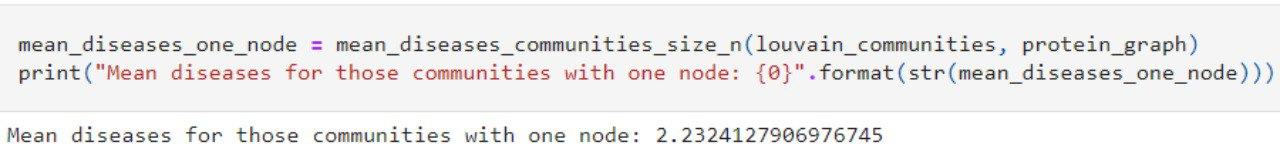
\includegraphics[width=1\linewidth]{images/singletons_mean_size.jpg}}\\
    \subfloat[Average community size \label{subfig:mean_community_size}]{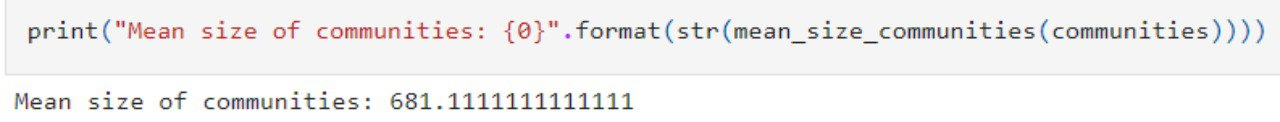
\includegraphics[width=1\linewidth]{images/community_mean_size.jpg}}
    \caption{Number of diseases for single-gene communities and mean size of kept communities.}
    \label{fig:mean_diseases_nodes_communities}
\end{figure}
Such communities were then plotted with the pyvis package\footnote{https://github.com/WestHealth/pyvis} by assigning different colors to better visualize them as we can see from \autoref{fig:communities}, we highlighted the SON gene by giving it a bigger size than all the other nodes in the graph. More graphs will be shown in \autoref{sec:results} to better illustrate the results.
\begin{figure}[H]
    \centering
    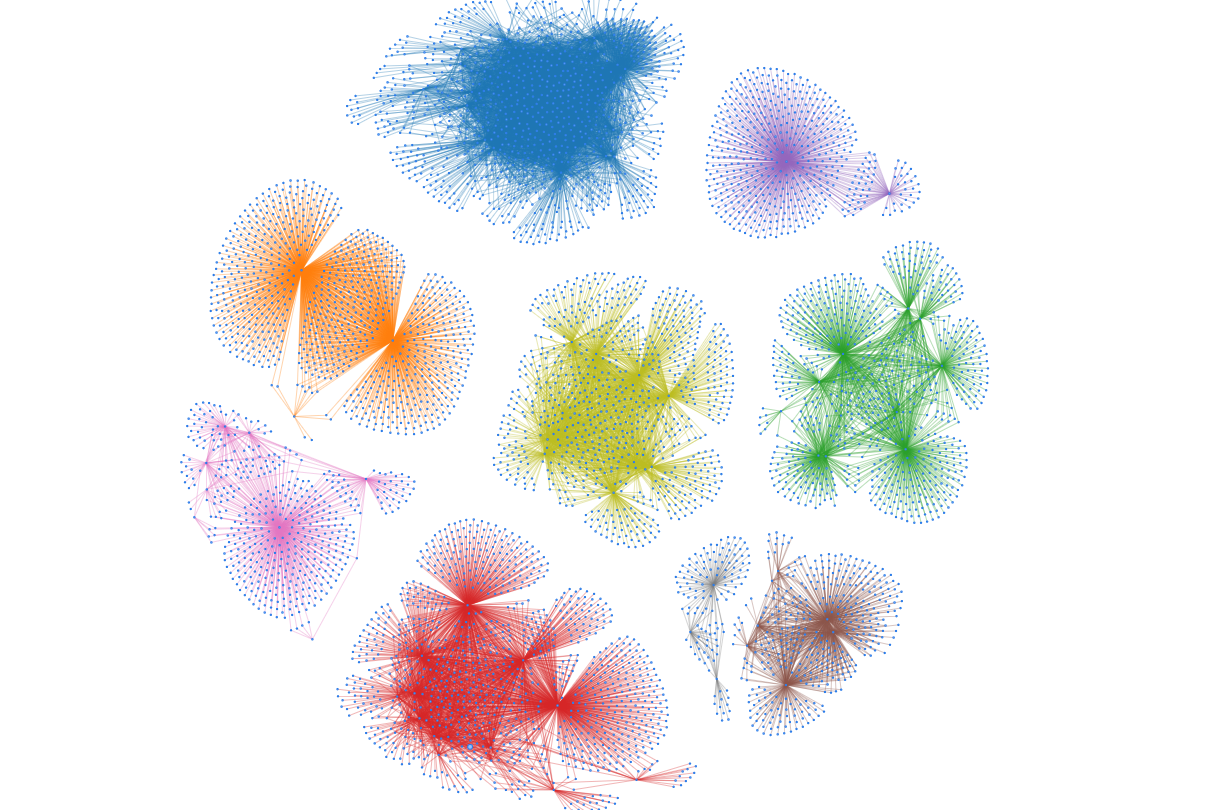
\includegraphics[width=0.9\linewidth]{images/plots/communities.png}
    \caption{Communities after the pruning.}
    \label{fig:communities}
\end{figure}

\subsection{Community evaluation}\label{subsec:community_evaluation}
In this section there will be the evaluation of the communities, which, in our example, there are $9$ of them (\autoref{fig:communities}). Every community contains a number of nodes which is involved in many different disease pathways and, to evaluate the goodness of the various clusters, we have implemented several metrics:
\begin{itemize}
    \item \textbf{Ratio disease}, measuring the ratio between the genes of the given community which participate to a disease pathway over the whole size of that pathway. This metric is particularly useful to avoid that the largest pathways are always the major contributors of the community. For example the "Malignant neoplasm of breast", which has around 3400 genes, without this metric would be the most relevant disease in almost every community. Scaling it with its size, gives a better perspective of its actual contribution in the interval $(0,1]$.
    \begin{equation}
        R_d = \frac{n_c}{n_d}
        \label{eq:ratio_disease}
    \end{equation}
    \item \textbf{Ratio community}, again a ratio, this time between the number of genes in a given pathway over the size of the community.This other metric puts in relation the contribution of every pathway in a given community with the community size, rewarding pathways with a lot of contribution in the community and has value in the interval $(0,1]$, this metrics solves the problem with small pathways entirely contained in the same community.
    \begin{equation}
        R_c = \frac{n_c}{|V_c|}
    \end{equation}
    \item \textbf{Relevance}, represents the best of both worlds. It combines the absolute contribution of the pathway with the community size, and is obtained multiplying the previous 2 metrics. It has, again, values in the interval $(0,1]$. 
    \begin{equation}
        Relevance = R_d \times R_c
    \end{equation}
\end{itemize}
\begin{figure}[H]
    \centering
    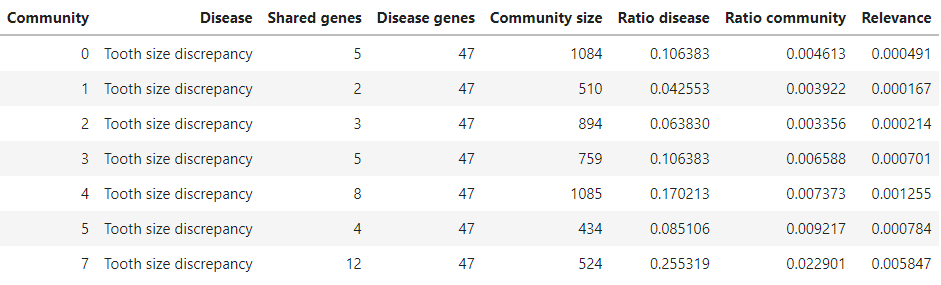
\includegraphics[width=1\linewidth]{images/disease_community_metrics.png}
    \caption{The community-disease dataframe with the computed metrics, we choose a disease as an example.}
    \label{fig:disease_community_metrics}
\end{figure}
By taking into account the computed metrics we can also determine the distance of every community to all the other ones. Since the distance is based on disease-related metrics, it also represents a similarity value between the communities.For our purpose this metric is not relevant since we needed to focus only on the SON community, but it could be useful for future improvement of an hypothetical pathway analysis package.
\begin{figure}[H]
    \centering
    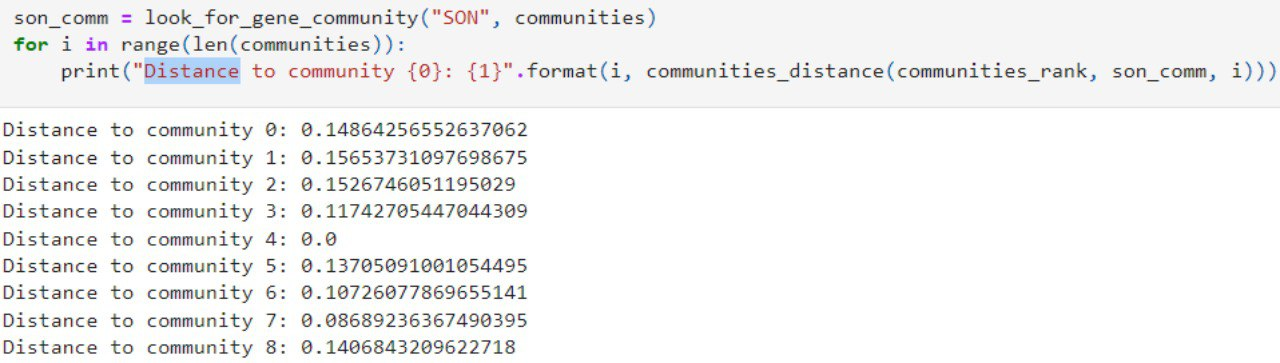
\includegraphics[width=0.8\linewidth]{images/distance_communities.jpg}
    \caption{Distance between the SON gene's community towards the other ones, the lower the value the better.}
    \label{fig:distance_communities}
\end{figure}